%document describing teh final version of ny dosse response model and what I think about its fit. Writen by Faith, started Augst 21st 2020.
\documentclass[11pt,letter]{article}
\usepackage[top=1.00in, bottom=1.0in, left=1.1in, right=1.1in]{geometry}
\renewcommand{\baselinestretch}{1.1}
\usepackage{graphicx}
\usepackage{natbib}
\usepackage{amsmath}
\usepackage{textcomp}%amoung other things, it allows degrees C to be added
\usepackage{float}
\usepackage{hyperref}
\usepackage[utf8]{inputenc} % allow funny letters in citaions 
\usepackage[nottoc]{tocbibind} %should add Refences to the table of contents?
\usepackage{amsmath} % making nice equations 

\def\labelitemi{--}
\parindent=0pt

\title{Winegrape Hardiness \\ My final (I hope) dose response model}
\date{\today}
\author{Faith Jones}

\graphicspath{ {./DoseResponse_WriteupImages/} }% tell latex where to find photos 


\begin{document}
%\renewcommand{\refname}{\CHead{}}%not sure what this was supposed to do 
\renewcommand{\bibname}{References}%names reference list 


\maketitle{}
\tableofcontents

\section{Background}
Dose response curves are regression models. The exact form of dose response models varies somewhat, encompassing a range of different statistical models including nonlinear regression models, generalized regression and parametric survival analyses \cite{Ritz2015}. What connects these models is their application: to model the effect of some dose on a biological response. The model assesses the relationship between what is traditionally named the ``dose'' or ``concentration'' and the ``response'' or ``effect''. This terminology comes from the model's  original use in pharmacology for modeling the effects of substances on physiology. The dose is usually some sort of biological stress that elicits a response from a biological organism. Dose values should be non-negative \cite{Rudemo1989} and the response values should change monotonically with increasing dose. Variations on the dose-response model have been applied to a wide variety of ecological questions, including species richness responses to nitrogen \cite{Jones2018a}, eco-toxicology \cite{Haanstra1985}, and phenology (winegrape budburst dates) \cite{Kovaleski2019}. \\

My analyses focus on sigmoid curve log-logistic models. These models are used to model relationships between variables with asymptotic minimum and maximum response values. I use the four parameter log-logistic model described in \cite{Ritz2015} and the below section, where the relationship between the dose and the response is a function of a maximum response, a minimum response, a response rate, and a dose giving a 50\% response. A benefit of this model is that the parameters are easily interpretable and biologically meaningful \cite{Seefeldt2016}\\

\section{Model Structure}
\subsection {Basic Model}

As introduced above, I use a four parameter log-logistic model to model winegrape cold hardiness (Equation \ref{eq1}). We used mean 2 day air temperature for our modeling because \textbf{Check Carl's reasoning} and because winegrape hardiness is closely linked to mean air temperatures \cite{Hubackova1996}. Air temperature readings were taken at \textbf{Penticton agCanada site??? check}. \\

Some modifications to the original data are needed, though, before analysis. Firstly, to ensure the dose values are always positive, I added 30 to each air temperature value. Secondly, I multiplied the hardiness values with \-1 so that larger values in the model meant higher winter hardiness. This was to make interpreting the minimum and maximum asymptotes of the model more intuitive. \\

\begin{equation} \label{eq1}
\mu=f(x,(b,c,d,e))=c+\frac{d-c}{1+exp^{b(log(x)-\tilde{e})}} 
\end{equation}
\begin{equation}
\label{eq:2}
\tilde{y}_{i}\sim normal(\mu_{i},\sigma)
\end{equation}

Where:
\begin{itemize}
\item[]	$x$ is the concentration of the dose (amount of winter cold) \\
$b$ is the response rate (slope)\\
$d$ is the upper asymptote of the response (maximum hardiness)\\
$c$ is the lower asymptote of the response (minimum hardiness)\\
$e$ is the effective dose ED50 (winter temperature where cold hardiness is half way between min and max)  \\
$\tilde{e}$ is the log of the effective dose ED50\\
\end{itemize}

\subsection {Full Model}

The final model includes hierarchical variance for different varieties and sites on the $d$ (maximum hardiness) parameter and for variety on the $b$ (rate of change) parameter (Equation \ref{modelWithPriors}) \\

We expected different sites to vary in their maximum hardiness because the model uses temperature data for a single site but the weather conditions at sites in the Okanagan Valley can vary substantially. For example (\textbf{insert name of site}) is a site on a south facing slope close to the lake shore and so is warmer, whereas the colder site of (\textbf{insert name of site}) is further north and more inland. Such micro-climatic differences should cause maximum hardiness to be less in warmer sites and more in colder sites. \\

Winegrapes have been domesticated for many thousands of years, and over that time growers have cultivated a wide range of varieties (genetically unique variants) with different physiological and ecological characteristics. Winegrape varieties consequently vary a lot in many of their traits. Although the exact mechanisms behind winegrape winter hardiness are unknown, winter hardiness seems to vary across varieties \cite{Mills2006,Ferguson2014,Kovaleski2018a}. Winegrapes may have different rates of change of winter hardiness\cite{Kovaleski2018a,Ferguson2014} and different maximum hardiness values \cite{Ferguson2014}. We included a hierarchical effect of variety on both maximum hardiness and the rate of change of hardiness so we could assess how variable variety specific winter hardiness is. \\

We built our dose response model in a Bayesian framework using Stan \textbf{cite stan version} in R \textbf{cite rstan and r}. An essential part of modeling using Bayesian methods is the choice of prior expectations on each parameter value. Our priors are specified in Equation \ref{modelWithPriors}, and were generally chosen to encompass all possible parameter combinations according to our current physiological understanding of winegrape hardiness. The exception to this is parameter $c$, minimum winter hardiness. Our data did not span the full range of the sigmoid curve relationship of winter hardiness to air temperature; we lack data on minimum hardiness. This is a problem for model estimating. An estimation of minimum hardiness of winegrapes was taken from a selection of sources: -3\textdegree C \cite{Ferguson2011}, -1.2\textdegree C \cite{Ferguson2014} \textbf{more sources}. We fed this estimation into the model as a prior constrained closely around -2\textdegree C.  

\begin{equation}
\label{modelWithPriors}
\mu=f(x_{i},(b,c,d,e))=c+\frac{(d+d_{var,i} + d_{site,i}) -c}{1+exp^{b_{var}(log(x_{i})-\tilde{e})}}
\end{equation}
\begin{equation}
{d}_{var} = dr_{var} * \sigma_{dvar}
\end{equation}
\begin{equation}
{d}_{site} = dr_{site} * \sigma_{dsite}
\end{equation}
\begin{equation}
{b}_{var} = br_{var} * \sigma_{bvar}
\end{equation}
\begin{equation}
\tilde{y}_{i}\sim normal(\mu_{i},\sigma)
\end{equation}

Where:
\begin{itemize}
\item[]$x$ is the concentration of the dose (amount of winter cold) \\
$b$ is the response rate (slope)\\
$d$ is the grand upper asymptote of the response (maximum hardiness hardiness) 
$d_{var}$ is the effect of each variety on the upper asymptote of the response (maximum hardiness)\\
$d_{site}$ is the effect of each site on the upper asymptote of the response (maximum hardiness)\\
$\sigma_{dvar}$ is the standard deviation of the effect of varieties on maximum winter hardiness\\
$\sigma_{dsite}$ is the standard deviation of the effect of sites on maximum winter hardiness\\
$dr_{var}$ is the non centred parameterization values for varieties effect on maximum hardiness d\\
$dr_{site}$ is the non centred parameterization values for sites effect on maximum hardiness d\\
$b$ is the lower asymptote of the response (minimum hardiness)\\
$\sigma_{bvar}$ is the standard deviation of the effect of varieties on rate of change of winter hardiness\\
$br_{var}$ is the non centred parameterization values for varieties effect on rate of change\\
$e$ is the effective dose ED50 (winter temperature where cold hardiness is half way between min and max)  \\
$\tilde{e}$ is the log of the effective dose ED50\\
\end{itemize}

Priors:\\
(hardiness has been multiplied with -1 to be positive, and 30 has been added to air temp)
\begin{itemize}
\item[]$b \sim gamma(7,1)$\\
$\sigma_{bvar} \sim normal(0,3)$ \\
$br_{var} \sim normal(0,1)$ \\
$d \sim Normal(25, 10)$ \\
$\sigma_{dvar} \sim gamma(2.5,1.75)$ \\
$dr_{var} \sim normal(0,1)$ \\
$\sigma_{dsite} \sim gamma(2.5,1.75)$ \\
$dr_{site} \sim normal(0,1)$ \\
$c \sim normal(2,0.5)$\\
$\tilde{e} \sim normal(log(30), 0.15)$ \\
$\sigma \sim normal(0,5)$\\
\end{itemize}

See Figure \ref{fig:parameters} for graphical representations of these distributions. \\

\begin{figure}
  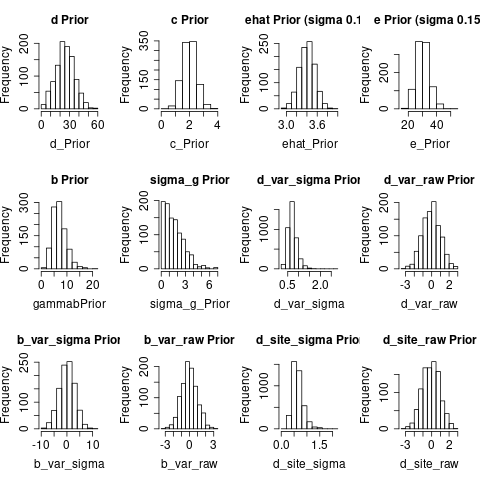
\includegraphics[scale = 1]{Priors.png}
  \caption{The parameter prior distributions used in the dose response model}
  \label{fig:parameters}
\end{figure}

\section{Model fit}
\subsection{Prior Predictive Checks}
I used Stan's generate quantities block with fixed parameters to undertake the prior predictive check. The potential parameter space defined by these parameters (Figure \ref{fig:priorPredictions}) allows only for a positive relationship between hardiness and air temperature because we know physiologically that winegrapes do not get less cold hardy as air temperate drops. No relationship is possible but unlikely as we know that winegrapes do acquire winter hardiness. Minimum hardiness is generally kept below 0\textdegree C, although some extreme values can reach above 0. The vast majority of sampling space though falls below 0 degrees hardiness, and I think this is good enough. Maximum hardiness can fall anywhere between 0\textdegree C and about -60\textdegree C, and is centered on -25\textdegree C because this is close to temperature I have seen quoted in the literature for more cold-hardy varieties \cite{Hubackova1996,Ferguson2014,Kovaleski2018a}. As mentioned above, the minimum hardiness is closely constrained around -2\textdegree C, but this constrain does not seem to cause the prior predictions to be too narrow.    

\begin{figure}
  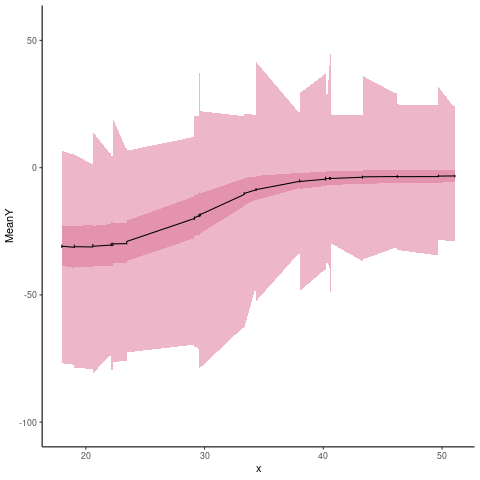
\includegraphics[scale = 0.5]{PriorPrediction.png}
  \caption{The potential winter hardiness according to the parameter space allowed by my priors. The black line is the mean predicted value of winter hardiness for each air temperature. The darker ribbon is the 25\% and 75\% bounds of the predicted values, and teh lighter ribbon is the most extreme values (1\% and 100\%).}
  \label{fig:priorPredictions}
\end{figure}

\subsection{Retrodictive Checks}
The model fits without any warning messages or the need for alterations to the fitting settings (adapt delta, tree-depth etc.). It runs with 2000 warm up steps and then 1000 iterations. The model generally does a good job I think of fitting to the data - most observed points fall withing the 89\% HPDI of the model predictions once hierarchical variation is considered \ref{fig:predWithReal}. There are some points though where the model overestimates hardiness. Most notably is a set of measurements at an air temperature of around -2\textdegree C that are obviously above the 89\%HPDI.  This cluster is also evident in when we plot the predicted values against the observed values (Figure \ref{fig:predAgainstReal}). These measurements come from a particularly cold day in November 2014 (Figure \ref{fig:2014Plot}).    

\begin{figure}
  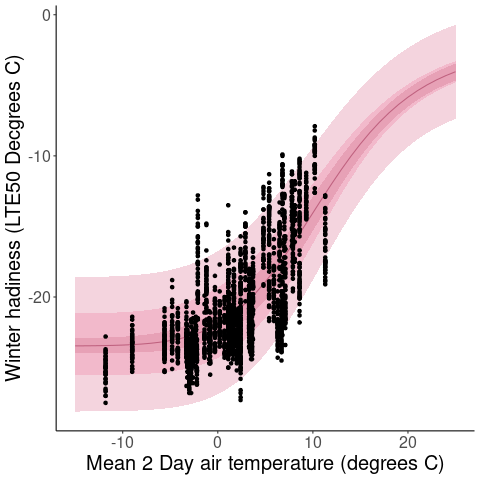
\includegraphics[scale = 0.5]{PredWithReal.png}
  \caption{The posterior estimations of the relationship between cold hardiness and air temperature, overlaid with the observed data. The line represents the mean prediction of the posterior, assuming to effect of variety or site. The bands around the line, from the lien outwards, are the 89\% HPDI around that mean prediction, the mean prediction with the mean effects of the most two most extreme varieties and sites, and the upper and lower 89\% HPDI of these estimates including extreme sites and varieties.}
  \label{fig:predWithReal}
\end{figure}

\begin{figure}
  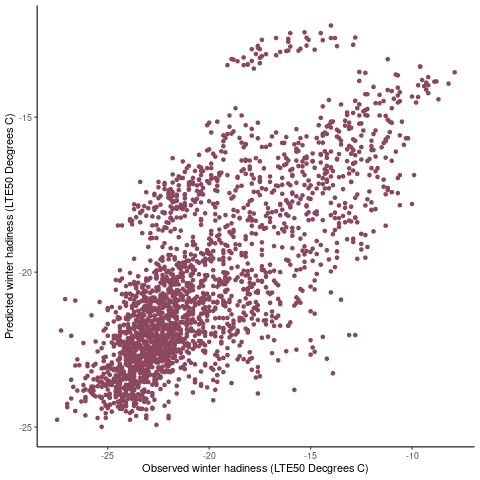
\includegraphics[scale = 0.5]{PredAgainstReal.png}
  \caption{The posterior estimations of the relationship between cold hardiness and air temperature plotted against the corresponding observed value}
  \label{fig:predAgainstReal}
\end{figure}


\begin{figure}
  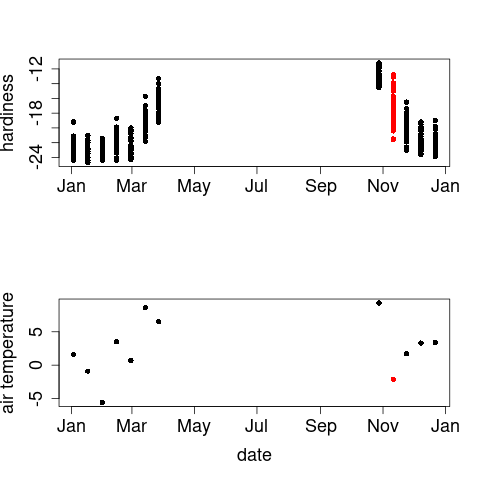
\includegraphics[scale = 0.75]{2014Data.png}
  \caption{The winter hardiness (above) and air temperature data (below) for 2014. Highlighted in red are data that the dose response model does not retrodict well. On this day the temperature was colder than usual for November. }
  \label{fig:2014Plot}
\end{figure}


\subsection{Estimated Parameter Values}
The model parameter estimations are shown in Figure \ref{fig:postParameters}. The maximum hardiness $(d)$ is around 23 \textdegree C, the 50\%dose rate (e) is around 10\textdegree C (40 in the figure but remember to take 30 from this value for the true air temperature value), the rate of change (b) us around 8, and general variance is a standard deviation of around 2.5\textdegree C. There is no noticeable hierarchical effect of variety on the rate of change as the highest probability parameter value for b\_var\_sigma is 0. There is an effect of variety and site on the maximum hardiness though. Both variety and site are estimated to have around 1\textdegree C effect and the effect of variety is estimated to be very slightly stronger (Figure \ref{fig:VarSiteD}). \\
The breakdown of individual varieties effect on maximum hardiness is shown in Figure \ref{fig:varDs}. Riesling was the most cold tolerant variety, and is closely followed by the Pinot varieties. Chardonnay was also more cold hardy than average. Viognier is also potentially cold more cold tolerant but a lack of much data means the model was more uncertain about this variety. Merlot, Gewurztraminer, Cabernet Franc and Sauvignon blanc were all less cold hardy than average, and Shiraz was the least cold hardy.  \\
Sites showed a similar level of variation to that of variety (Figure \ref{fig:siteDs}). The sites with the most cold hardy vines were Black Sage, Oliver-east. OK Falls-east, and Osoyoos-southeast. Vines at Olver-west, Kelowna and West Kelowna were all less cold hardy than average. Vines at Osoyoos-west and OK Falls-west were of middling hardiness. \\
There is no discernible difference between the rate of change of hardiness (b) of different vine varieties (Figure \ref{fig:varBs}). This is to be expected because the model did not suggest an effect of variety on the rate of change (b) parameter.


\begin{figure}
  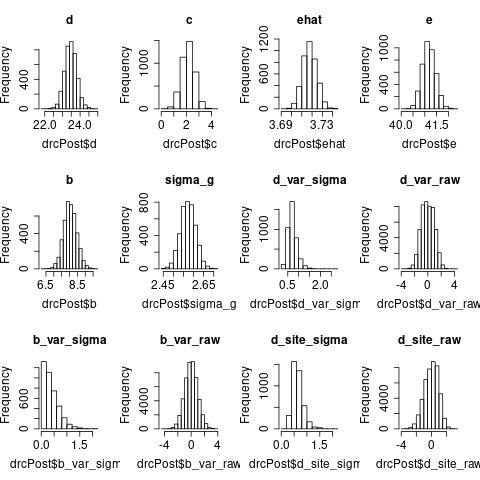
\includegraphics[scale = 0.75]{Parameters.png}
  \caption{The posterior estimations of the parameters in the dose response model}
  \label{fig:postParameters}
\end{figure}

\begin{figure}
  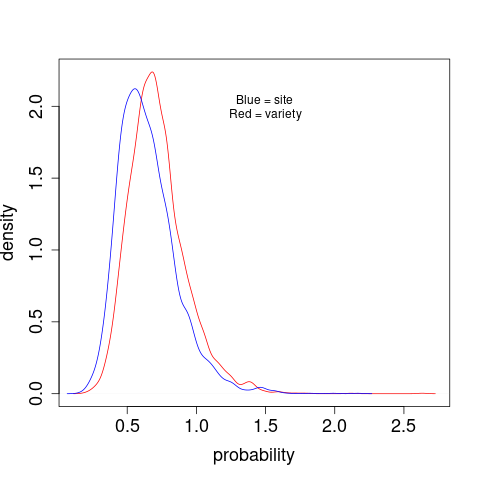
\includegraphics[scale = 0.75]{VarSiteD.png}
  \caption{The posterior distribution of the parameters describing the effect of variety (in red) and site (in blue) on maximum winter hardiness (d).  }
  \label{fig:VarSiteD}
\end{figure}

\begin{figure}
  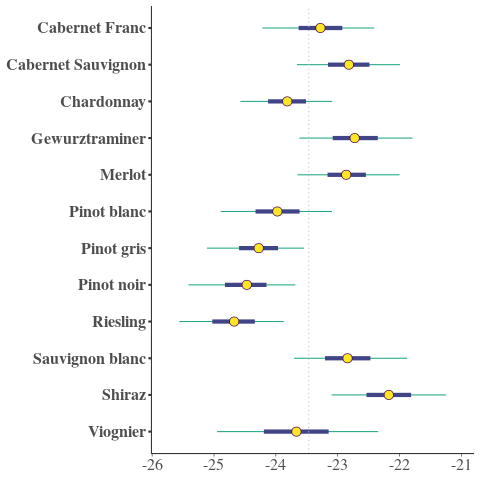
\includegraphics[scale = 0.75]{varDs.png}
  \caption{The variation in maximum hardiness (d) of each variety.The gray dotted lien represents the mean maximum hardiness (d).}
  \label{fig:varDs}
\end{figure}

\begin{figure}
  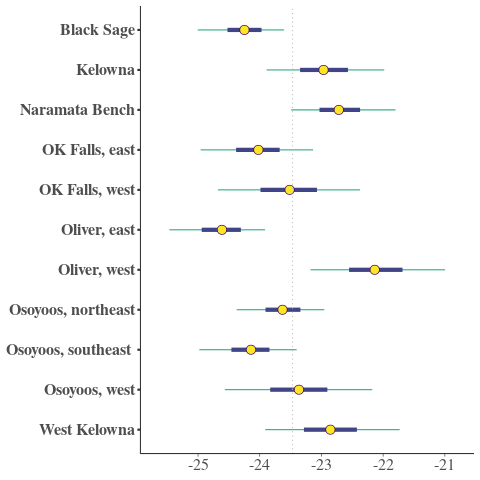
\includegraphics[scale = 0.75]{siteDs.png}
  \caption{The variation in maximum hardiness (d) of each site.The gray dotted line represents the mean maximum hardiness (d).}
  \label{fig:siteDs}
\end{figure}

\begin{figure}
  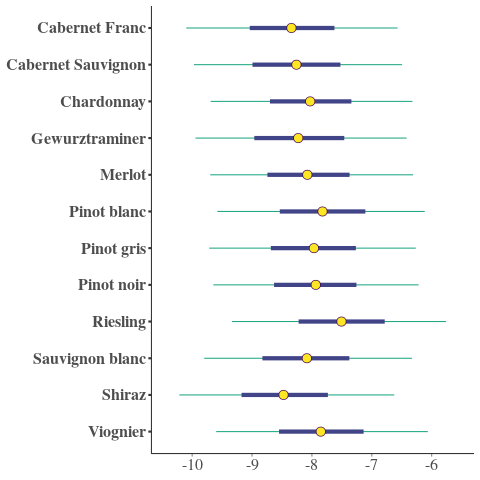
\includegraphics[scale = 0.75]{varBs.png}
  \caption{The variation in rate of change of hardiness (b) of each variety.The gray dotted lien represents the mean rate of change of hardiness (b).}
  \label{fig:varBs}
\end{figure}



\subsection{Predictions}
We set out to build a model that could estimate the cold hardiness of vines based on the air temperature. To check that this model does that I decided to see how well it predicted data from a new source. For this exercise I used winter hardiness of Cabernet Sauvignon grown at the Irrigated Agriculture Research Extension Center (IAREC) in Prosser, WA, USA and published by \cite{Ferguson2014} in the on-line version of their hardiness model. These data are gathered in a similar way to our Okanagan training data; canes are taken from the field to the laboratory where LTE values are extracted using DTA. \\

To gain model predictions I used the generated quantities section of the Stan model block. This involved feeding a new set of x values into the model that was mot used in the model fitting section. because this was a new site which I had no prior knowledge of, I kept the effect of site on d as 0. I used the Cabernet Sauvignon effect on maximum hardiness though. \\

The model does a fairly good job of predicting winter hardiness in this new dataset despite it being from a different location (Figure \ref{fig:WashingtonPredictionxy})  . Most observed values fall within the quartile range of predictions, with the notable exception of an overestimated value at around 2\textdegree C. This value fell on a particularly cold autumn day; the temperatures before and after were above 10\textdegree C. In general the model is more accurate at predicting winter hardiness in colder (sub 0) air temperatures (Figure \ref{fig:WashingtonPredictionyy}). \\



\begin{figure}
  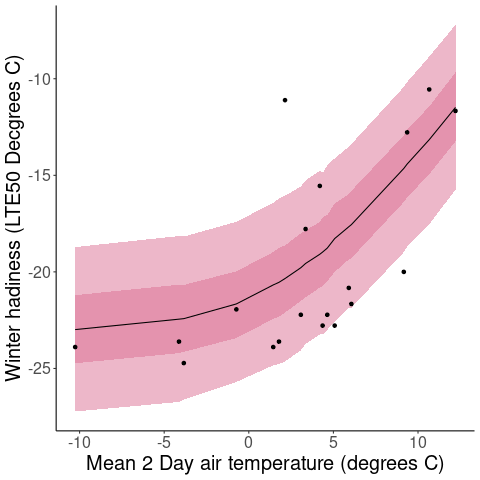
\includegraphics[scale = 0.75]{WashingtonPrediction.png}
  \caption{The observed winter hardiness of Cabernet sauvignon at the Washington State experimental plot, overlaid with the predicted winter hardiness of this variety using our mode. The line is the mean prediction, the darker band is the 25\% and 75\% quartile predictions, and the lighter band is the 5\% and 75\% predictions.   }
  \label{fig:WashingtonPredictionxy}
\end{figure}

\begin{figure}
  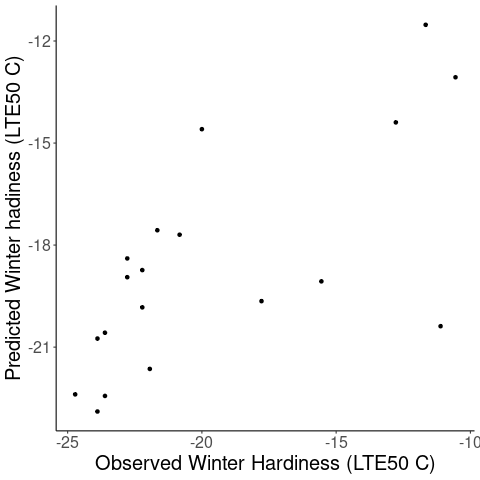
\includegraphics[scale = 0.75]{WashingtonPrediction2.png}
  \caption{The observed winter hardiness of Cabernet sauvignon at the Washington State experimental plot plotted against the observed data for each temperature. }
  \label{fig:WashingtonPredictionyy}
\end{figure}

\subsection{1 day mean temperatures}
I tried the model with 1 day mean temperature which I calculated using todays minimum temperatures and yesterday's maximum temperature. The plot looks a little odd (Figure \ref{fig:OneDayPredxyDRC}). For some reason with the 1 day temperatures there are more coasions where hardiness is qhite a bit lower than the model predicts. Maybe 3 day average woudl work even better, if the averaging helps smooth out those unusually cold days that currently throw the model? The model did not fit as well in terms of the parameter posteriors (Figure \ref{fig:OneDayPairsDRC}) and I got lost of warning red text after Stan finished running. For some reason there is multimodality in the parameter posteriors, thsi is probably teh reason for all the model fit problems.  

\begin{figure}
  \includegraphics[scale = 0.75]{OneDayPredxyDRC.png}
  \caption{The variation in rate of change of hardiness (b) of each variety.The gray dotted lien represents the mean rate of change of hardiness (b).}
  \label{fig:OneDayPredxyDRC}
\end{figure}


\begin{figure}
  \includegraphics[scale = 0.75]{OneDayPairsDRC.png}
  \caption{The variation in rate of change of hardiness (b) of each variety.The gray dotted lien represents the mean rate of change of hardiness (b).}
  \label{fig:OneDayPairsDRC}
\end{figure}

\subsection{multimodality in the posteriors }
I tried to recreate the multi-modality i was seeing in some of the earlier models. The only prior combination I successfully found with this multi-modality was when I did not restrict b to be positive. There were two sets of values, one for positive slopes and one for negative slopes. Otherwise the problem with posteriors was mostly in the co-linearity between ehat and c.  




\section{Discussion}

Generally the model seems to do a good job of predicting values, even from new datasets/areas. I was pretty happy with how it predicted the data from Washington State, especially when the vines approach maximum winter hardiness. There are some issues though around cold snaps in the autumn when the model expects winegrapes to be more cold hardy than they are. I assume cold snaps in the spring might cause similar problems? I am not sure how much of a problem this flaw is for winegrape growers though, because the air temperatures are nowhere near the vines LTE50 at the time when the model is mis-estimating. In the two cases highlighted in this document the air temperatures were not below -2\textdegree C, and while the vines were not as hardy as predicted they were still a good 10\textdegree C more hardy than the air temperature. Still, perhaps I should focus more on maximum hardiness and really cold snaps rather than late/early cold snaps? \\

The differences the model picks up for variety maximum hardiness generally agree with values in the literature (Figure \ref{fig:compareFerg}). Our estimations are generally for more winter hardy vines than that of \cite{Ferguson2014} though, especially for Merlot, Chardonnay and Sauvignon blanc. I am not really sure why this is, especially when out model predicted maximum hardiness well for their Cab franc data. Maybe we could try some of their other hardiness data and see if the model is less good for Merlot or Chardonnay?\\
Or result of no effect of variety on the rate of change of hardiness is at odds with that of \cite{Ferguson2014}. I need to look closer at \cite{Kovaleski2018a,Kovaleski2019} to see how their results compare with ours. Some quick thoughts though - does our model suggest that all varieties are similarly vulnerable to unseasonably warm or cold weather because they will all react at the same rate? So for example Chardonnay won't lose hardiness quicker than Riesling in the spring? But then how do some of teh most hardy varieties manage to lose hardiness and budbreak early enough?\\

\begin{figure}
  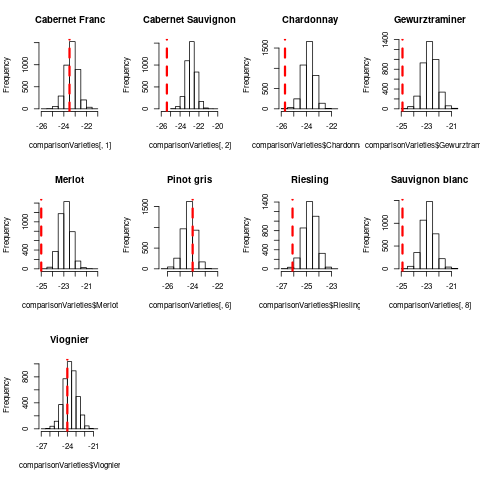
\includegraphics[scale = 0.75]{compareFerg.png}
  \caption{A comparison between the maximum winter hardiness predicted by our dose repose model in comparison to \cite{Ferguson2014}'s dynamic model. To aid in comparison the histograms show the posterior probabilities of the effect of each variety plus the mean predicted maximum hardiness. Red vertical lines are the estimations from the literature. }
  \label{fig:compareFerg}
\end{figure}

Is Shiraz the newest addition to the Okanagan? Will it be grown more as temps increase? This thought comes from the fact that it is the least hardy variety. \\

How important is the sigma\_g result (about 2 \textdegree C)? Is that too much uncertainty for the growers? What about the uncertainty in model predictions? Is our model actually functional?\\


Site differences - how do these compare to our (Carl's) knowledge of the geography of the sites?\\


Compare relative importance of variety and site for growers adapting to climate change. \\

\bibliographystyle{/home/faith/Documents/Bibtex/styles/besjournals/besjournals}



\bibliography{/home/faith/Documents/Bibtex/mendeleyStuff/library}

\end{document}

